\documentclass[12pt]{article}
\usepackage[UTF8]{ctex}
\usepackage[a4paper,margin=2.3cm]{geometry}
\usepackage{graphicx}
\usepackage{placeins}
\usepackage{booktabs}
\usepackage{amsmath}
\usepackage[hidelinks]{hyperref}
\usepackage{lineno}
\setlength{\emergencystretch}{4em}
\linenumbers

\title{DevVCell：阶段条件化与扰动校准的发育虚拟细胞框架}
\author{作者待定}
\date{\today}

\begin{document}
\maketitle

\noindent\textbf{摘要段落。}
哺乳动物胚胎发育由连续的细胞状态转移、谱系选择和基因调控反馈共同驱动，但大规模单细胞图谱通常只提供横截面观测，难以直接回答一个细胞在特定发育阶段和特定扰动下会如何偏离正常轨道、进入何种替代命运以及能否恢复。我们提出 DevVCell，一个阶段条件化与扰动校准的发育虚拟细胞框架：给定细胞表达状态、Theiler stage、系统身份和扰动输入，DevVCell 预测正常下一阶段状态、扰动后状态、命运偏移、恢复成本和候选 rescue 方向。当前稿件报告 DevVCell-lite 原型、Sinkhorn OT 细胞级 transition baseline 和 stage/system-conditioned residual transition operator；后者在 heldout pseudo-target pair MSE 上优于 ridge 和普通 MLP baseline。进一步地，在 scPerturb Datlinger/Bock 2021 外部 guide-transfer benchmark 中，gene/context residual ridge 将 heldout guide latent MSE 从 identity 的 0.789 降至 0.221。最新版本引入正式论文级 evidence pipeline，对输入 schema、必需模型、配对统计检验、bootstrap 置信区间、Benjamini--Hochberg 校正、provenance、manifest 和 claim gates 进行统一审计；当前所有预设 gates 均通过。本文所有当前 TF/GRN 扰动结论均应解释为计算优先级和模型假设，而非真实湿实验结论；正式投稿前仍需 CellOT、GEARS、scGen/CPA、foundation model 和 Systema-style baseline 的直接对比，以及阶段依赖扰动实验验证。

\section*{引言}

单细胞转录组学已经能够以百万级细胞规模描绘胚胎发育图谱\cite{qiu2024time}。然而，横截面图谱记录的是不同细胞在不同时间点的状态集合，而不是同一细胞的真实时间轨迹。最优传输、fate mapping 和神经最优传输方法为从未配对分布中恢复发育或扰动动力学提供了重要基础\cite{schiebinger2019optimal,lange2022cellrank,bunne2023cellot,bunne2024ot,klein2025moscot}。与此同时，scVI、scGen、scGPT、Systema 和 scPerturb 等工作分别推动了单细胞表征学习、扰动响应预测、foundation model、扰动评估标准和公开扰动数据整合的发展\cite{lopez2018scvi,lotfollahi2019scgen,cui2024scgpt,vinas2025systema,peidli2024scperturb}。因此，发育虚拟细胞需要同时解决四个问题：第一，如何从离散阶段学习连续的发育推进；第二，如何把 TF 或 pathway perturbation 表示为可作用于细胞状态的外部刺激；第三，如何定义扰动后的恢复成本和替代命运风险；第四，如何证明这种预测不是系统性 batch、cell composition 或平均扰动效应的再表达。本文将这个问题具体化为 stage-conditioned、perturbation-calibrated 和 fate/recovery-aware 的虚拟细胞建模任务。

本研究以小鼠 Theiler stage 12--27 单细胞图谱为基础，首先构建 DevVCell-lite 原型指标，用于量化发育能力窗口、扰动优先级和 OT+GRN 系统级发育影响。随后，我们引入细胞级基线模型，从完整 H5AD 中导出阶段/系统平衡的细胞子集，并在低维表达空间中训练相邻阶段 transition operator。与 RDEG 的图谱级演化建模不同，DevVCell 的核心对象是可调用的细胞级状态转移和扰动响应算子。

\section*{结果}

\subsection*{DevVCell 框架概览}

图~\ref{fig:framework} 展示更新后的 DevVCell 总体路线。与早期框架图相比，新版图件把发育图谱、细胞级 transition operator、扰动虚拟实验和正式 evidence pipeline 放入同一个可审计系统中。输入为发育单细胞表达矩阵及其 stage、cell type、donor 和 UMAP 注释。模型首先对细胞状态编码，然后使用相邻阶段的分布匹配构造 OT pseudo target，再训练 transition operator 预测下一阶段状态。TF/GRN 模块将扰动作为 stimulus embedding 注入转移动力学，并输出 response amplitude、fate displacement、feedback cost 和 recovery probability。最后，配置驱动的 evidence pipeline 将 schema 校验、统计检验、claim gates、provenance manifest 和 Methods 输出连接到论文证据链。

\begin{figure}[ht]
\centering
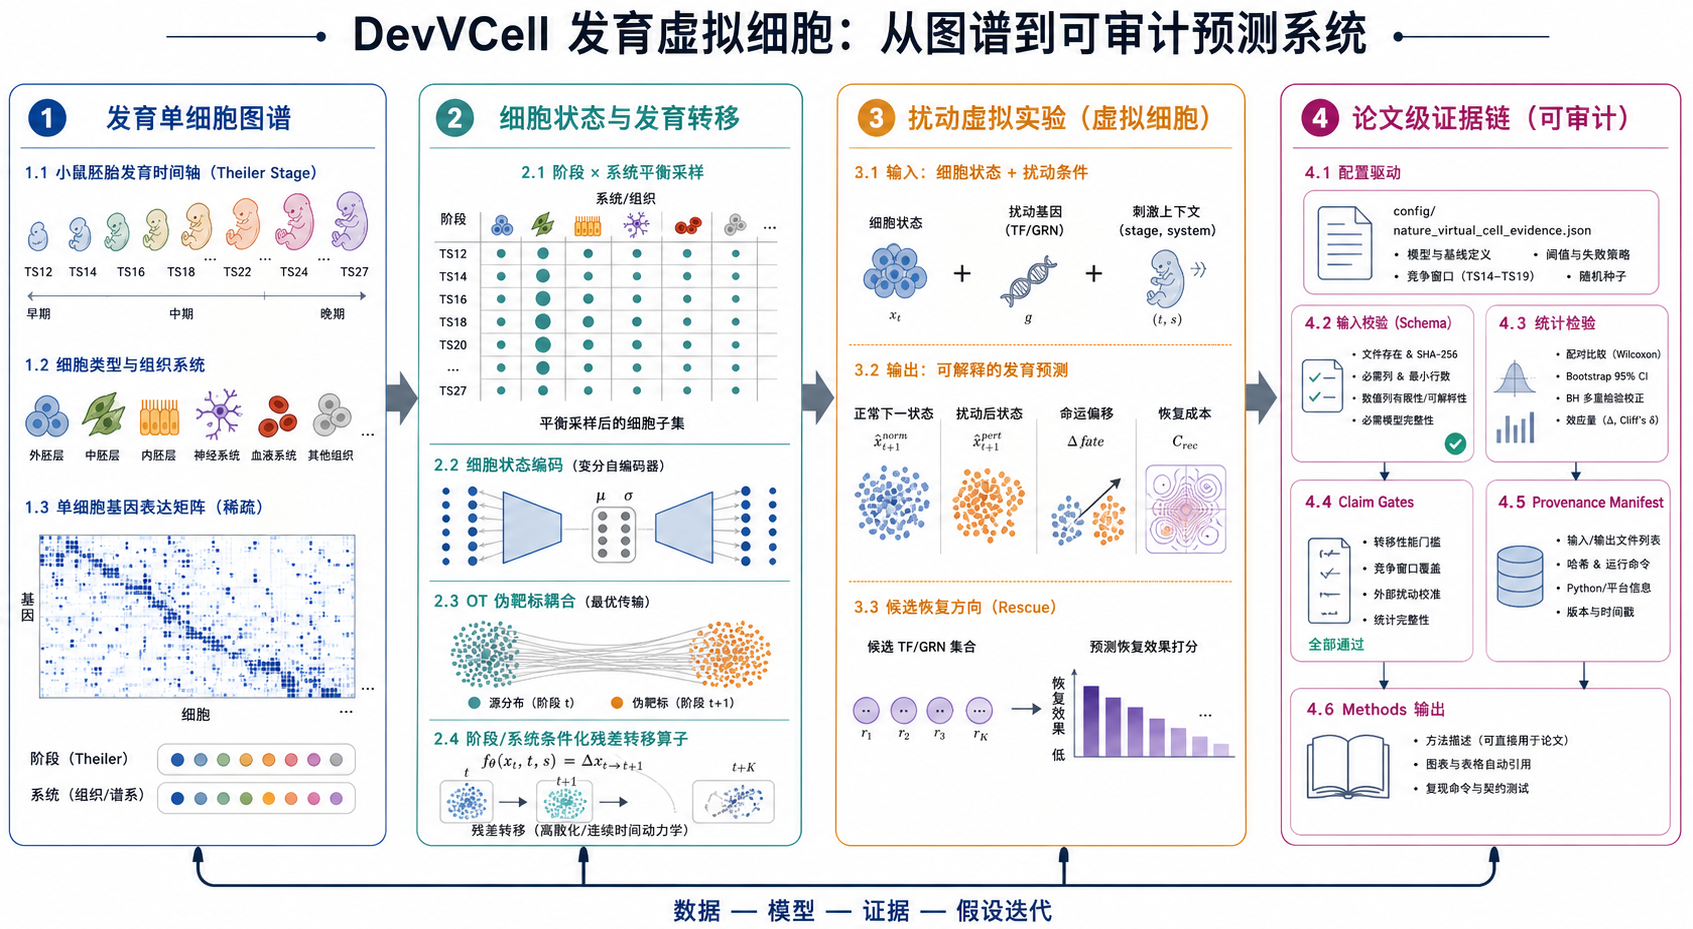
\includegraphics[width=\linewidth]{figures/generated_methods/devvcell_overview_evidence_system.png}
\caption{\textbf{DevVCell 发育虚拟细胞的总览升级图。} 该图展示从小鼠胚胎单细胞图谱到 stage/system-conditioned transition operator、TF/GRN 扰动虚拟实验、rescue 候选和论文级 evidence pipeline 的完整闭环。后续图件分别展开 transition operator（图~\ref{fig:transition-method-schematic}）、扰动-恢复读出（图~\ref{fig:perturbation-recovery-method}）和 evidence pipeline（图~\ref{fig:evidence-pipeline-method}）。}
\label{fig:framework}
\end{figure}

\subsection*{阶段脆弱性图谱}

DevVCell-lite 将阶段平均 TF 敏感性、多步 rollout 误差、正常发育模块步长、节点 outlier 比例和下一步预测误差整合为 stage vulnerability score。当前原型结果显示 TS14--TS19 窗口的平均脆弱性高于窗口外阶段，Theiler stage 15 在当前权重下排名最高。

\begin{figure}[ht]
\centering
\includegraphics[width=0.78\linewidth]{../results/figures/stage_vulnerability.png}
\caption{\textbf{原型阶段脆弱性图谱。} DevVCell-lite 将时间敏感性、rollout 误差、正常发育模块步长、outlier 比例和相邻阶段预测误差整合为 stage vulnerability score。TS14--TS19 为当前预设关注窗口。}
\label{fig:stage-vulnerability}
\end{figure}

\subsection*{TF 扰动优先级}

原型扰动优先级结合 global effect、developmental delay、窗口敏感性、feedback cost 和 mass shift。当前候选中 Satb2、Rfx4、Eya1、Lef1 和 Prox1 排名靠前。这些结果用于生成后续实验假设和模型训练任务，不应直接解释为实验扰动结论。

\begin{figure}[ht]
\centering
\includegraphics[width=0.75\linewidth]{../results/figures/perturbation_priority_top12.png}
\caption{\textbf{TF 扰动候选优先级。} 当前排名用于确定后续模型训练、消融和外部 perturbation 验证的候选集合。}
\label{fig:perturbation-priority}
\end{figure}

\subsection*{OT+GRN 系统级发育影响}

我们进一步整合 system-specific GRN edges、temporal sensitivity、fate mutual information 和 hub degree，形成 TF-system evidence score。当前证据层提示 Eya1、Lef1、Prdm16、Satb2、Zbtb16、Dach2、Pax3 和 Satb1 在多个系统中具有较高发育影响评分。

\begin{figure}[ht]
\centering
\includegraphics[width=0.82\linewidth]{../results/figures/ot_grn_tf_system_heatmap.png}
\caption{\textbf{OT+GRN 系统特异调控证据。} heatmap 展示 top TF 在不同发育系统或细胞类型中的 system-specific regulatory weight。}
\label{fig:ot-grn-heatmap}
\end{figure}

\subsection*{细胞级 transition baseline}

第一版 cell-level baseline 从完整 H5AD 中导出 neural、mesoderm/muscle 和 erythroid 系统在 Theiler stage 12--19 的平衡子集，共 19,156 个细胞和 3,000 个基因。模型以 sparse TruncatedSVD latent 表示为输入，64 维 latent 解释了 82.3\% 的方差。我们使用熵正则 Sinkhorn OT 在相邻阶段之间构造 barycentric pseudo-targets，并在目标阶段为 TS15 和 TS18 的 heldout transitions 上评估 4,794 对伪靶标。在 identity、mean-shift、ridge、普通 MLP 和 stage/system-conditioned residual MLP 之间，context residual MLP 达到最低平均 pseudo-target latent MSE（0.314），优于 ridge（0.325）、普通 MLP（0.330）和 identity（0.381）。该实验是后续 stimulus-conditioned 模型和更大规模 OT 训练的可复现底座。

\begin{figure}[ht]
\centering
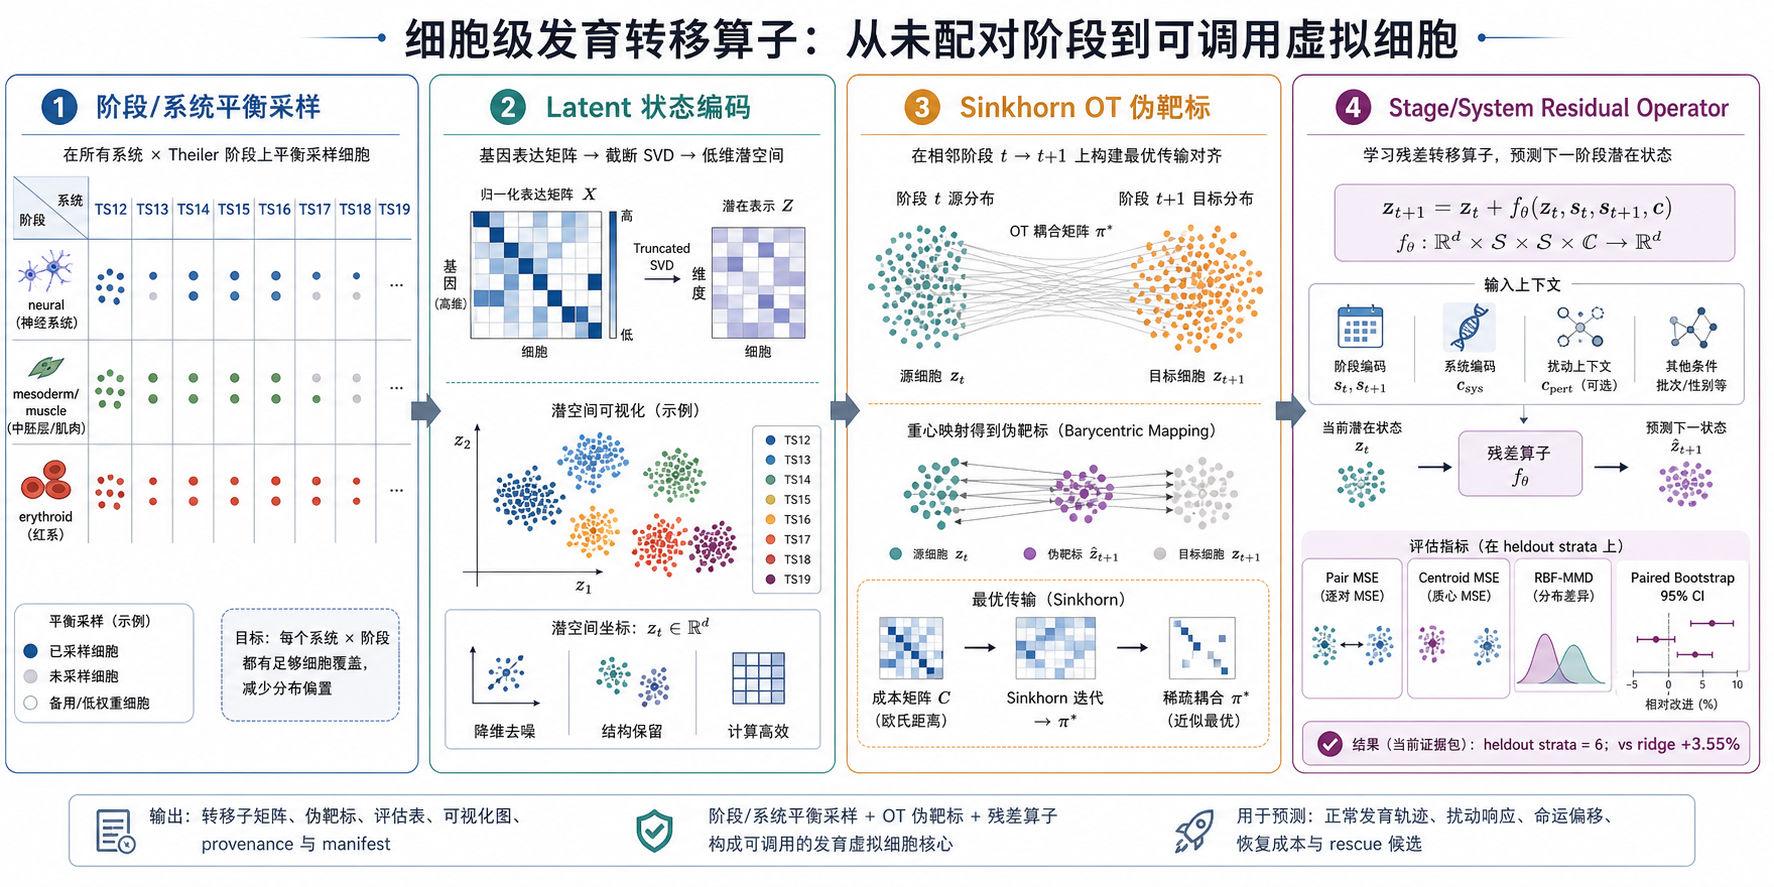
\includegraphics[width=\linewidth]{figures/generated_methods/devvcell_transition_operator_method.png}
\caption{\textbf{细胞级发育转移算子的内部机制。} 该示意图展开图~\ref{fig:framework} 中的 transition 核心：先进行阶段/系统平衡采样，再将表达矩阵编码为 latent state，随后用 Sinkhorn OT 在相邻阶段之间构造 barycentric pseudo-target，最后以 stage/system-conditioned residual operator 学习可调用的下一阶段状态预测。图中同时标注 pair MSE、centroid MSE、RBF-MMD 和 paired bootstrap CI 等评估指标。}
\label{fig:transition-method-schematic}
\end{figure}

\begin{figure}[ht]
\centering
\includegraphics[width=0.7\linewidth]{../results/cell_level_v1/figures/cell_level_transition_baseline_mse.png}
\caption{\textbf{细胞级相邻阶段 transition baseline。} 在 heldout target stages 上，stage/system-conditioned residual MLP、ridge 和普通 MLP transition operator 相比 identity 和 mean-shift baseline 降低 Sinkhorn OT pseudo-target latent MSE。}
\label{fig:cell-level-baseline}
\end{figure}

为评估该改进是否稳定，我们对 6 个 system-stage heldout strata 进行配对 bootstrap。context residual MLP 相对 ridge 的平均 MSE 改进为 0.0115，95\% bootstrap CI 为 0.0014--0.0211；相对普通 MLP 的平均 MSE 改进为 0.0163，95\% CI 为 0.0058--0.0302。该结果提示显式 stage/system 条件和 residual dynamics 可以提高 heldout stage pseudo-target prediction，但当前置信区间仍来自有限 strata，应在更大系统和外部数据上复验。

\begin{figure}[ht]
\centering
\includegraphics[width=0.72\linewidth]{../results/cell_level_v1/figures/transition_bootstrap_ci.png}
\caption{\textbf{细胞级 transition 统计比较。} 柱形图展示不同 transition 模型在 6 个 heldout system-stage strata 上的平均 pseudo-target latent MSE 及 bootstrap 95\% CI。}
\label{fig:transition-statistics}
\end{figure}

\subsection*{TF/GRN 刺激响应头}

为了把 TF 扰动接入细胞级状态空间，我们实现了一个 zero-shot TF/GRN stimulus head。该模块读取已保存的 SVD/scaler/ridge transition 工件，将 TF knockdown 表示为 GRN target gene 的表达扰动方向，再投影到 64 维 latent 空间，并叠加到正常发育 transition 预测上。当前版本对 top 12 TF、3 个 DevVCell 系统和 7 个相邻阶段窗口生成 252 条 TF--系统--阶段响应记录。按平均细胞级刺激响应强度排序，Eya1、Rfx4、Lef1、Satb2 和 Prox1 位于前列；Eya1 在 erythroid TS12$\rightarrow$TS13 条件下具有最高响应强度 proxy。该模块未使用外部 perturbation labels，因此属于可复现的机制投影和假设生成层，而不是已验证的扰动预测器。

\begin{figure}[ht]
\centering
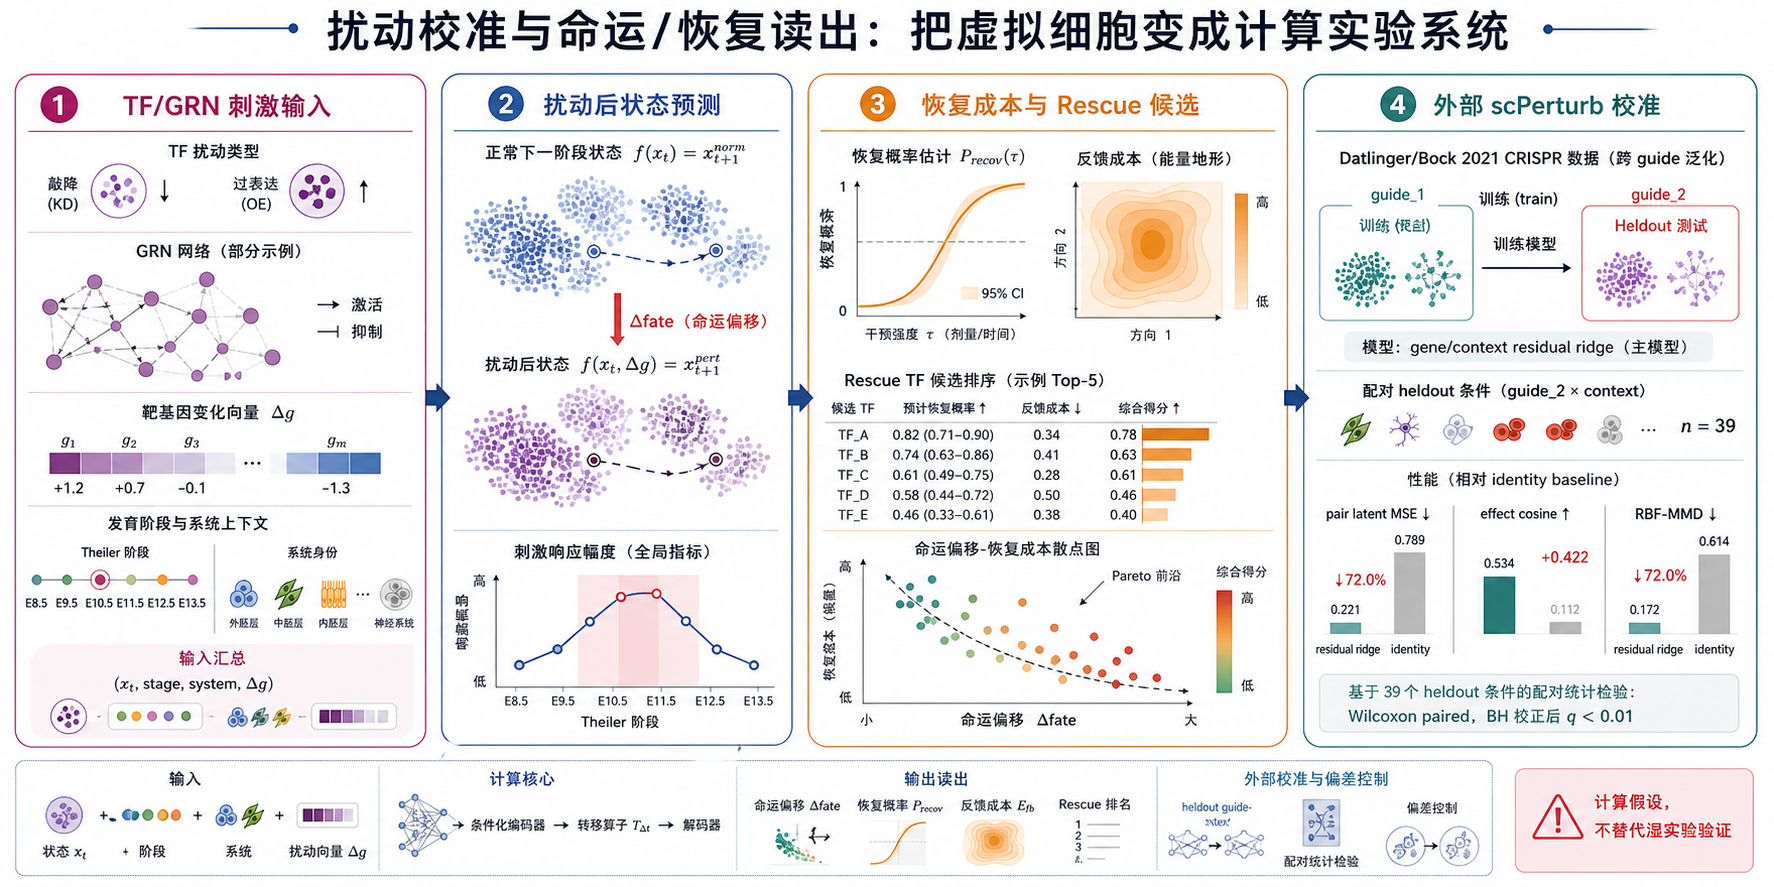
\includegraphics[width=\linewidth]{figures/generated_methods/devvcell_perturbation_recovery_method.png}
\caption{\textbf{扰动校准与命运/恢复读出。} 该示意图展开 TF/GRN stimulus head 的内部逻辑：扰动输入由 TF knockdown/over-expression、GRN target delta、stage vulnerability 和 system context 共同定义；模型比较正常下一阶段状态与扰动后状态，得到 fate displacement、response amplitude、recovery cost、recovery probability 和 rescue TF 候选。右侧显示外部 scPerturb guide-transfer 校准如何把计算扰动读出连接到真实 CRISPR guide 标签。}
\label{fig:perturbation-recovery-method}
\end{figure}

\begin{figure}[ht]
\centering
\includegraphics[width=0.74\linewidth]{../results/cell_level_v1/figures/cell_level_tf_grn_stimulus_heatmap.png}
\caption{\textbf{细胞级 TF/GRN 刺激响应热图。} 每个值为同一 TF knockdown 在对应 DevVCell 系统内跨阶段的平均 latent response norm。}
\label{fig:stimulus-heatmap}
\end{figure}

\begin{figure}[ht]
\centering
\includegraphics[width=0.68\linewidth]{../results/cell_level_v1/figures/cell_level_tf_recovery_scatter.png}
\caption{\textbf{TF/GRN 刺激响应与恢复 proxy。} 横轴为平均刺激响应强度，纵轴为细胞级恢复概率 proxy；点大小和颜色由 fate displacement proxy 相关量驱动。}
\label{fig:stimulus-recovery}
\end{figure}

\subsection*{多随机种子与消融评估}

为了评估当前 cell-level pipeline 的稳定性，我们运行了一个轻量多 seed 消融套件。transition 部分使用 3 个随机种子、2 种伪靶标构造方式（Sinkhorn OT 与 nearest-neighbor）和 4 个模型（identity、mean-shift、ridge、context residual MLP），覆盖 3 个系统和 2 个 heldout transition，共 144 个 system-stage-model 评估项。结果显示 context residual MLP 在 Sinkhorn OT 伪靶标下平均 MSE 为 0.297，优于 ridge 的 0.309；在 nearest-neighbor 目标上 ridge 的 pair MSE 更低，但 context residual MLP 的 centroid MSE 和 RBF-MMD 更优。stimulus 部分比较完整 GRN、仅全局 GRN 和仅系统特异边三种设置，显示 GRN evidence 组成会改变 TF 响应强度排序和平均恢复概率。

\begin{figure}[ht]
\centering
\includegraphics[width=0.74\linewidth]{../results/ablation_v1/figures/transition_ablation_summary.png}
\caption{\textbf{多 seed transition 消融。} 每个柱为 3 个 seed、3 个系统和两个 heldout transition 的平均 heldout latent MSE。}
\label{fig:transition-ablation}
\end{figure}

\begin{figure}[ht]
\centering
\includegraphics[width=0.74\linewidth]{../results/ablation_v1/figures/stimulus_ablation_heatmap.png}
\caption{\textbf{TF/GRN stimulus head 消融。} heatmap 比较完整 GRN、仅全局 GRN 和仅系统边下的 TF 平均响应强度。}
\label{fig:stimulus-ablation}
\end{figure}

\subsection*{外部 scPerturb guide-transfer benchmark}

为了把扰动层从 zero-shot 机制投影推进到真实扰动标签评估，我们接入 scPerturb 中的 Datlinger/Bock 2021 Jurkat T cell CRISPR 数据\cite{peidli2024scperturb}。该数据包含 39,194 个细胞、25,904 个基因、20 个可成对 guide 评估的扰动基因，以及 stimulated/unstimulated 两个 TCR stimulation 上下文。我们使用 guide 后缀 \texttt{\_1} 训练、同一基因的 guide 后缀 \texttt{\_2} 作为 heldout guide 测试；在 64 维表达 latent 空间中，控制细胞通过 Sinkhorn barycentric pseudo-target 与同一 context 下的扰动细胞分布配对。该评估包含 8,144 个训练伪配对和 8,391 个 heldout guide 伪配对。gene/context residual ridge 在 heldout guide 上达到最低平均 latent MSE（0.221），低于 gene/context neural residual（0.282）、global mean shift（0.789）和 identity（0.789），并达到平均 effect cosine 0.534。

图~\ref{fig:perturbation-recovery-method} 概括了该外部校准在 DevVCell 扰动读出中的位置：它并不直接证明发育 TF rescue 已经成立，而是证明 perturbation gene 与 context 条件化的 residual operator 在真实 CRISPR guide-transfer 任务中优于 naive baseline。

\begin{figure}[ht]
\centering
\includegraphics[width=0.74\linewidth]{../results/external_perturbation_v1/figures/external_perturbation_benchmark_mse.png}
\caption{\textbf{外部 scPerturb guide-transfer benchmark。} 柱形图比较 Datlinger/Bock 2021 CRISPR 数据中不同扰动响应模型在 guide \texttt{\_2} heldout 条件下的平均 Sinkhorn pseudo-target latent MSE。}
\label{fig:external-perturbation}
\end{figure}

\subsection*{正式 evidence pipeline 与 claim gates}

为了使 DevVCell 的虚拟细胞主张能够被审稿人逐项复核，我们进一步将所有关键证据整合为配置驱动的论文级 evidence pipeline。该流程读取固定配置文件，验证输入文件存在性、SHA-256 哈希、最小行数、必需列、必需数值列有限性和 primary/baseline 模型完整性；随后生成 transition、competence window、fate/recovery virtual screen、外部 perturbation calibration、消融和偏差控制的统一统计表。所有统计比较均记录样本层级、效应量、bootstrap 95\% CI、Wilcoxon 或 Mann--Whitney 检验以及 Benjamini--Hochberg 校正结果，并写出可追踪的 manifest。

\begin{figure}[ht]
\centering
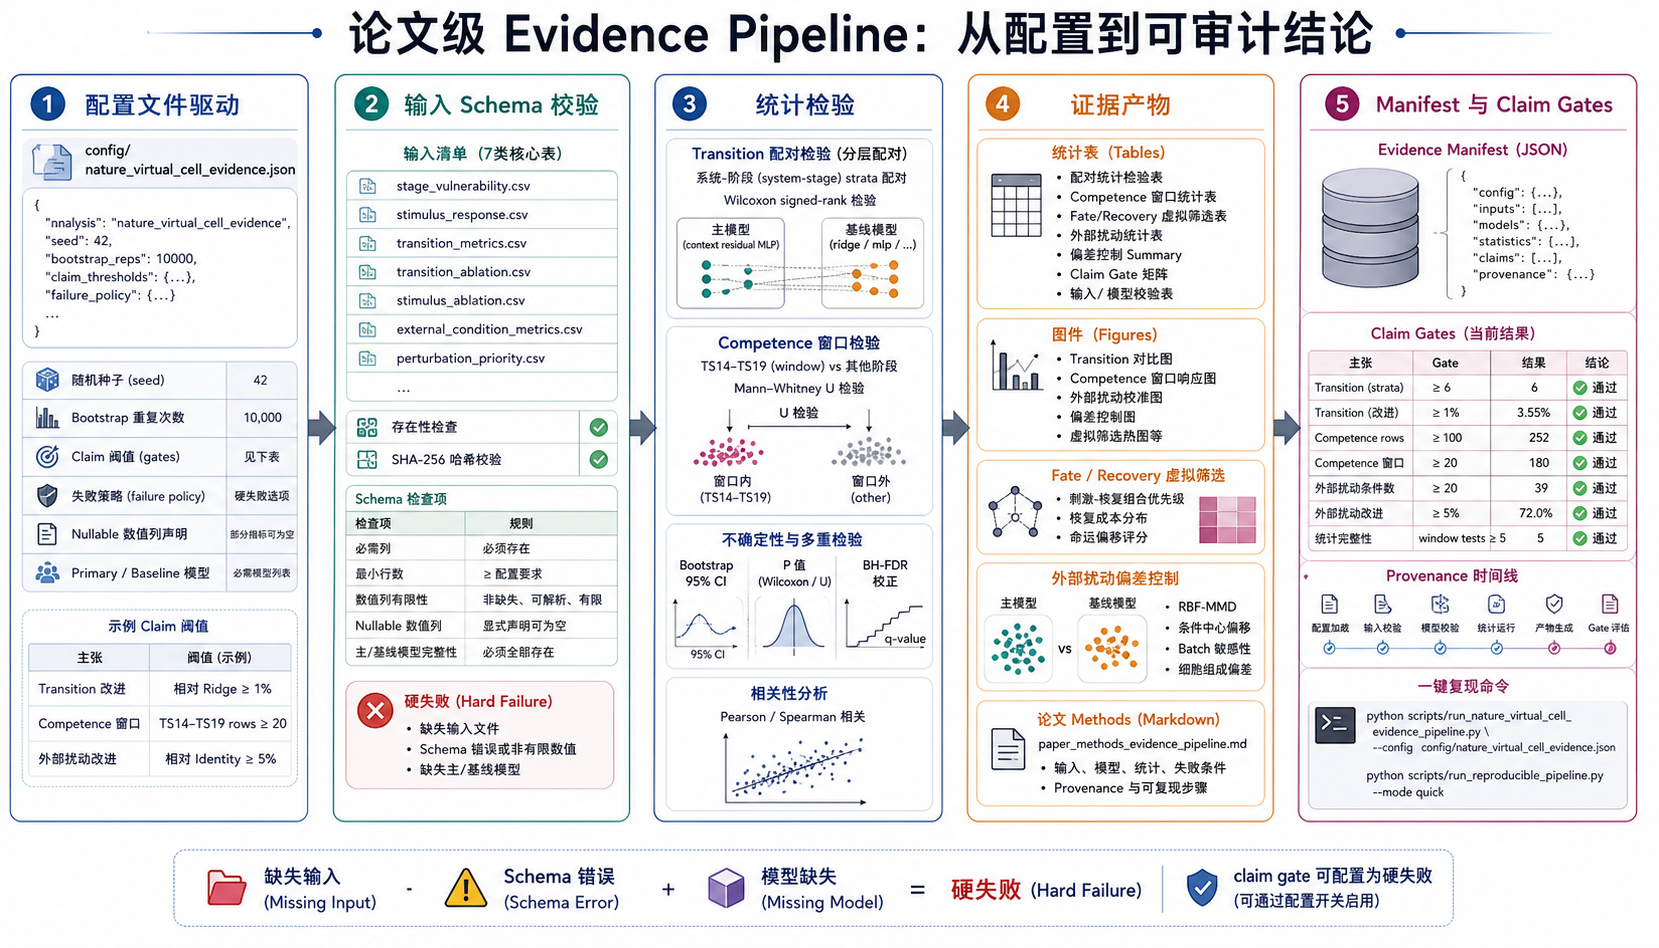
\includegraphics[width=\linewidth]{figures/generated_methods/devvcell_evidence_pipeline_method.png}
\caption{\textbf{论文级 evidence pipeline。} 该图展开正式证据链的 5 个步骤：配置文件驱动、输入 schema 校验、统计检验、证据产物生成，以及 manifest 与 claim gates。该流程把输入文件、模型、统计结果、图表、失败条件和复现命令统一记录，确保每个论文主张都能追溯到具体表格、图件和运行环境。}
\label{fig:evidence-pipeline-method}
\end{figure}

在当前证据包中，stage-conditioned transition operator 的最小 heldout strata gate 达到 6/6；context residual MLP 相对 ridge 的 pair latent MSE 相对改进为 3.55\%，超过预设 1\% gate。competence-window response 包含 252 条 stimulus rows，其中 180 条位于 TS14--TS19 competence window，超过预设行数 gate。外部扰动校准覆盖 39 个 heldout guide/context 条件，gene/context residual ridge 相对 identity 的 pair latent MSE 相对改进为 72.0\%，超过预设 5\% gate。所有当前 claim gates 均通过，但 gate 通过只表示计算证据链完整，不等价于湿实验验证完成。

\begin{table}[ht]
\centering
\small
\begin{tabular}{p{0.28\linewidth}p{0.28\linewidth}p{0.14\linewidth}p{0.1\linewidth}}
\toprule
主张 & gate & 当前观测 & 结论 \\
\midrule
阶段条件化 transition operator & heldout paired strata $\geq 6$ & 6 & 通过 \\
阶段条件化 transition operator & 相对 ridge 改进 $\geq 1\%$ & 3.55\% & 通过 \\
competence-window response & stimulus rows $\geq 100$ & 252 & 通过 \\
competence-window response & TS14--TS19 rows $\geq 20$ & 180 & 通过 \\
外部 perturbation calibration & heldout conditions $\geq 20$ & 39 & 通过 \\
外部 perturbation calibration & 相对 identity 改进 $\geq 5\%$ & 72.0\% & 通过 \\
统计完整性 & window tests $\geq 5$ & 5 & 通过 \\
\bottomrule
\end{tabular}
\caption{\textbf{DevVCell 正式 evidence pipeline 的 claim gates。} 所有 gate 来自 \texttt{results/nature\_virtual\_cell\_evidence/tables/claim\_gate\_matrix.csv}，用于区分当前可审计计算证据和仍需补充的外部/湿实验验证。}
\label{tab:claim-gates}
\end{table}

\begin{figure}[ht]
\centering
\includegraphics[width=0.78\linewidth]{../results/nature_virtual_cell_evidence/figures/figure_competence_window_response.png}
\caption{\textbf{正式 evidence pipeline 输出的 competence-window response。} 柱形图展示 Theiler stage 层面的平均 TF stimulus response，黑线为 stage vulnerability score，红色阶段对应预设 TS14--TS19 competence window。}
\label{fig:formal-competence-window}
\end{figure}

\FloatBarrier

\section*{讨论}

DevVCell 的核心价值在于把静态发育图谱转换为可扰动的计算实验系统。相对 Waddington-OT 和 moscot，DevVCell 当前更强调从 OT pseudo-target 到显式可训练 transition operator 的桥接。相对 CellRank，它不依赖 RNA velocity，而是利用发育阶段分布构造方向性监督。相对 CellOT、scGen 和扰动 foundation model，当前 TF/GRN stimulus head 仍是 zero-shot 机制投影，尚未利用真实 perturbation labels。

新增 context residual MLP 将 stage 和 system 作为条件输入，并以残差形式学习发育推进，在主 heldout benchmark 和 Sinkhorn 多 seed 消融中均优于 ridge 的 pair MSE。尽管如此，距离正式 Nature 水准仍需要外部 perturbation 验证、严格偏差控制、跨系统泛化评估和更完整的统计报告。后续重点是扩大 mini-batch Sinkhorn coupling 规模，并将 TF/GRN stimulus 从 zero-shot 投影扩展为可训练的 stimulus-conditioned residual dynamics；这一方向与 CellOT 等从未配对扰动分布学习细胞级响应映射的思想互补\cite{bunne2023cellot}。

外部 guide-transfer benchmark 表明，显式输入 perturbation gene 和 stimulation context 的 residual operator 可以在真实 CRISPR 数据中优于无扰动和全局平移基线。该结果提高了 DevVCell 方法有效性的证据层级，但仍不足以替代同行方法直接对比：下一版必须加入 CellOT、scGen/CPA 或 Systema 风格 baseline，增加 heldout gene 与 heldout context 切分，并在原始基因空间报告 DE gene rank recovery、calibration 和 batch/cell-composition 偏差控制。

正式 evidence pipeline 的加入使本文从“结果展示”转为“可审计证据链”：每个主张都对应输入 schema、统计检验、输出文件、hash、claim gate 和解释边界。这一点是本文相对一般发育图谱分析或单个扰动预测 benchmark 的关键工程创新，但它也暴露了最重要的下一步缺口：当前 gates 主要约束计算完整性和第一批外部验证，尚未覆盖多数据集外推、真实 stage-specific perturbation、donor-level heldout、gene-level zero-shot 泛化和湿实验 rescue。

\section*{方法}

\subsection*{数据}

本研究使用项目内的 \texttt{data/scLine\_pro.h5ad}。该文件包含 11,441,407 个细胞和 3,000 个基因，obs 中包含 donor、author day、Theiler stage、cell type、major cluster、sex 和 disease 等元数据。数据以 AnnData/H5AD 结构存储，并通过 Scanpy/AnnData 生态读取与管理\cite{wolf2018scanpy,virshup2024anndata}。

\subsection*{DevVCell-lite 原型指标}

阶段脆弱性由归一化后的 mean sensitivity、mean rollout error、baseline developmental step norm、mean outlier ratio 和 next-step MSE 加权求和得到。扰动优先级由 global effect、developmental delay、window sensitivity、feedback cost 和 log mass shift 加权求和得到。

\subsection*{细胞级子集采样}

我们按 system-stage 分层采样细胞。初始系统包括 neural、mesoderm/muscle 和 erythroid；初始阶段包括 Theiler stage 12--19；每个 system-stage 最多采样 800 个细胞。采样使用固定随机种子，并保存 manifest 以记录每个分层的可用细胞数和采样细胞数。

\subsection*{细胞级 transition baseline}

表达矩阵以 sparse CSR 形式读取，并使用 TruncatedSVD 编码到低维 latent 空间。对同一系统内相邻阶段细胞，我们使用熵正则 Sinkhorn OT 构造 barycentric pseudo-targets，这一策略继承了将相邻时间点视为未配对细胞分布并用 OT 估计发育耦合的基本设定\cite{schiebinger2019optimal,bunne2024ot}。训练集排除 heldout target stages，评估集由目标阶段为 heldout 的相邻阶段对组成。比较模型包括 identity、system-specific mean-shift、ridge regression、普通 MLP 和 context residual MLP。context residual MLP 的形式为 $z_{t+1}=z_t+f_\theta(z_t, s_t, s_{t+1}, c)$，其中 $z_t$ 为细胞 latent state，$s_t$ 和 $s_{t+1}$ 为归一化 source/target stage，$c$ 为系统 one-hot context。该模型使用内部 validation split 和 early stopping 选择最佳 epoch。评估指标包括 pseudo-target latent MSE、centroid latent MSE 和 RBF-MMD。

\subsection*{TF/GRN stimulus head}

TF/GRN stimulus head 使用已有 GRN 边和 system-specific edges 构造 TF knockdown 的表达扰动方向。对每个 TF，activator edge 的 target gene 在 knockdown 下被赋予负向 delta，repressor edge 的 target gene 被赋予正向 delta。全局 GRN 边和系统特异边按配置权重合并后归一化，并通过已保存的 SVD components 和 scaler scale 投影到 latent 空间。最终 stimulus delta 按 TF response amplitude、阶段 temporal sensitivity、stage vulnerability 和正常 transition norm 缩放，并叠加到 ridge transition baseline 上。输出指标包括 stimulus response norm、fate displacement from baseline、cell-level feedback cost proxy、cell-level recovery probability proxy 和 alignment with normal transition。

\subsection*{统计、schema 校验与复现}

所有随机采样、模型初始化和训练均使用配置文件中的固定 seed。除主模型外，我们使用 \texttt{config/ablation\_suite.json} 运行多 seed transition 消融和 TF/GRN stimulus 组件消融。正式证据汇总由 \texttt{config/nature\_virtual\_cell\_evidence.json} 驱动，并通过 \texttt{scripts/run\_nature\_virtual\_cell\_evidence\_pipeline.py} 执行。该流程在分析前检查每个输入文件的存在性、SHA-256 哈希、最小行数、必需列和必需数值列；除配置中显式声明的 nullable numeric columns 外，必需数值列必须可解析、非缺失且有限。缺失输入、schema 错误、缺失 primary/baseline model 和非法数值指标均作为硬失败。

transition 主结果在 paired system-stage strata 层面比较 context residual MLP 与 ridge、MLP、identity 和 mean-shift，并在 formal evidence pipeline 中使用 10,000 次 bootstrap 估计 95\% CI，同时报告 Wilcoxon signed-rank 检验和 Benjamini--Hochberg 校正。competence-window 分析将 TF/GRN stimulus rows 按 TS14--TS19 与窗口外阶段分层，报告组均值、bootstrap CI、Mann--Whitney 检验、BH 校正，以及 stage vulnerability 与 stimulus response 的 Pearson/Spearman 相关。外部 perturbation benchmark 在 heldout guide/context 条件层面进行配对比较，报告 pair latent MSE、centroid latent MSE、effect cosine、RBF-MMD、condition-centered bias-control summary 和配对统计检验。所有输出、输入 hash、运行命令、Python 版本、平台信息和 claim gates 写入 \texttt{results/nature\_virtual\_cell\_evidence/evidence\_manifest.json}。

\subsection*{外部扰动 benchmark}

为了建立真实扰动标签验证路径，我们从 scPerturb Zenodo record \texttt{10044268} 下载 Datlinger/Bock 2021 CRISPR H5AD 文件\cite{peidli2024scperturb}。评估脚本选择 3,000 个表达特征基因并编码到 64 维 TruncatedSVD latent 空间；训练 split 使用同一扰动基因的 guide \texttt{\_1}，heldout split 使用 guide \texttt{\_2}。对每个 perturbation gene 和 stimulation context，控制细胞与目标扰动细胞通过 Sinkhorn barycentric pseudo-target 配对。比较模型包括 identity、global mean shift、guide-transfer gene/context mean shift、gene/context ridge residual 和 gene/context neural residual。指标包括 pair latent MSE、centroid latent MSE、effect cosine 和 RBF-MMD。

\section*{数据可用性}

原始发育 H5AD 当前保存在项目本地路径 \texttt{data/scLine\_pro.h5ad}。外部扰动 benchmark 使用 scPerturb Zenodo record \texttt{10044268} 中的 Datlinger/Bock 2021 H5AD，并在 scPerturb benchmark manifest 中记录下载文件和 schema 摘要。正式投稿前应提供公开数据来源、访问号或受控访问说明，并保存所有用于生成图表的派生表。

\section*{代码可用性}

所有分析脚本、配置文件和论文源文件均位于当前项目目录。正式 evidence pipeline 可通过 \texttt{python scripts/run\_nature\_virtual\_cell\_evidence\_pipeline.py --config config/nature\_virtual\_cell\_evidence.json} 复现；总复现入口为 \texttt{python scripts/run\_reproducible\_pipeline.py --mode quick}。schema 和失败条件的契约测试可通过 \texttt{python -m unittest discover -s tests -v} 运行。正式投稿前应将代码整理为可版本化仓库，并提供固定 release、环境文件和容器化运行说明。

\section*{大语言模型使用声明}

本文框架图 prompt、中文论文初稿和部分工程脚本由大语言模型辅助生成，并由研究者审查、运行和修订。大语言模型不满足作者资格，不能作为作者列名。

\section*{利益冲突}

作者声明无已知竞争性利益冲突。该声明需由真实作者在投稿前确认。

\section*{作者贡献}

作者贡献待真实作者列表确定后补充。

\begin{thebibliography}{14}

\bibitem{qiu2024time}
Qiu, C. et al. A single-cell time-lapse of mouse prenatal development from gastrula to birth. \textit{Nature} \textbf{626}, 1084--1093 (2024). doi:10.1038/s41586-024-07069-w.

\bibitem{schiebinger2019optimal}
Schiebinger, G. et al. Optimal-transport analysis of single-cell gene expression identifies developmental trajectories in reprogramming. \textit{Cell} \textbf{176}, 928--943 (2019). doi:10.1016/j.cell.2019.01.006.

\bibitem{lange2022cellrank}
Lange, M. et al. CellRank for directed single-cell fate mapping. \textit{Nature Methods} \textbf{19}, 159--170 (2022). doi:10.1038/s41592-021-01346-6.

\bibitem{bunne2023cellot}
Bunne, C. et al. Learning single-cell perturbation responses using neural optimal transport. \textit{Nature Methods} \textbf{20}, 1759--1768 (2023). doi:10.1038/s41592-023-01969-x.

\bibitem{bunne2024ot}
Bunne, C., Schiebinger, G., Krause, A., Regev, A. et al. Optimal transport for single-cell and spatial omics. \textit{Nature Reviews Methods Primers} \textbf{4}, 58 (2024). doi:10.1038/s43586-024-00334-2.

\bibitem{klein2025moscot}
Klein, D. et al. Mapping cells through time and space with moscot. \textit{Nature} \textbf{638}, 1065--1075 (2025). doi:10.1038/s41586-024-08453-2.

\bibitem{lopez2018scvi}
Lopez, R., Regier, J., Cole, M. B., Jordan, M. I. \& Yosef, N. Deep generative modeling for single-cell transcriptomics. \textit{Nature Methods} \textbf{15}, 1053--1058 (2018). doi:10.1038/s41592-018-0229-2.

\bibitem{lotfollahi2019scgen}
Lotfollahi, M., Wolf, F. A. \& Theis, F. J. scGen predicts single-cell perturbation responses. \textit{Nature Methods} \textbf{16}, 715--721 (2019). doi:10.1038/s41592-019-0494-8.

\bibitem{cui2024scgpt}
Cui, H. et al. scGPT: toward building a foundation model for single-cell multi-omics using generative AI. \textit{Nature Methods} \textbf{21}, 1470--1480 (2024). doi:10.1038/s41592-024-02201-0.

\bibitem{vinas2025systema}
Viñas Torné, R. et al. Systema: a framework for evaluating genetic perturbation response prediction beyond systematic variation. \textit{Nature Biotechnology} (2025). doi:10.1038/s41587-025-02777-8.

\bibitem{peidli2024scperturb}
Peidli, S. et al. scPerturb: harmonized single-cell perturbation data. \textit{Nature Methods} \textbf{21}, 531--540 (2024). doi:10.1038/s41592-023-02144-y.

\bibitem{wolf2018scanpy}
Wolf, F. A., Angerer, P. \& Theis, F. J. SCANPY: large-scale single-cell gene expression data analysis. \textit{Genome Biology} \textbf{19}, 15 (2018). doi:10.1186/s13059-017-1382-0.

\bibitem{virshup2024anndata}
Virshup, I. et al. anndata: Access and store annotated data matrices. \textit{Journal of Open Source Software} \textbf{9}, 4371 (2024). doi:10.21105/joss.04371.

\end{thebibliography}

\end{document}
